\documentclass[journal]{IEEEtran}
\usepackage{cite}
\usepackage[dvips]{graphicx}
\usepackage{hyperref}

\begin{document}
\title{Optical phase characterization of integrated photonic devices}
\author{J.~Matres,~G.~C.~Ballesteros,~S.~Mas,~A.~Brimont,~P.~Sanchis,~J.~Mart\'i~and~C.~J.~Oton}
%\markboth{Journal of Lightwave Technology}%
%{Shell \MakeLowercase{\textit{J. Matres et al.}}: Optical phase characterization of integrated photonic devices}

\maketitle


\begin{abstract}
We propose a relatively simple experimental setup capable of accurately characterizing the optical phase response of an integrated photonic circuit. The setup is based on a phase-noise reduction scheme using an external heterodyne Mazch-Zehnder interferometer. In particular, we characterize the phase response of different silicon photonic components: undercoupled and overcoupled ring resonators, and a corrugated waveguide.
\end{abstract}

\section{Introduction}
\noindent In the last years, integrated optics has experimented a remarkable development thanks to technological advances but also because its recent trend towards standardization.
The main advantage of photonic integrated circuits is that one can build a extremely complex systems with hundreds of components on a very small footprint and at a very low cost per device.
The phase response of an element is a key parameter that is required for the design of a system which includes that element. However, measuring the phase response is not straightforward, as under normal circumstances phase noise prevents simple interferometric measurements using for example an external Mach-Zehnder interferometer (MZI).

Commercial devices sensitive to phase are typically referred to as \emph{optical vector network analyzer} (OVNA). These devices employ specific techniques to alleviate phase noise problems in their measurement, usually requiring very fast laser tuning speeds (in the order of 100~nm/s) and complex synchronous receiving schemes \cite{Vanwiggeren2003, Gifford2005}. Fast laser sweeping reduces phase noise, as thermally-induced noise usually has a 1/f spectral dependence.

In this work, we present a relatively simple setup which allows accurate and continuous phase response of the system by using an ordinary tunable laser with tuning speeds even below 1~nm/s.
The cancellation of phase noise is carried out by employing a counter-propagating reference beam at fixed wavelength.
This idea was applied in Ref.~\cite{Mas2012} to characterize chromatic dispersion in waveguides with different geometries.
This paper shows that the setup can be used to characterize the phase response of different building blocks, in particular, silicon micro-ring resonators and corrugated waveguides.
In the former, the measurement allowed us to distinguish undercoupling from overcoupling conditions.
In the latter, a detailed plot of the group index of the corrugation can be obtained from a single segment of waveguide without the need of integrated MZIs and fringe spacing calculations.


\section{Experimental setup}
The experimental setup is shown in Fig.~\ref{fig:dispersionSetup}.
It consists of a fiber-based MZI, where each branch has an acousto-optic modulator (AOM) which acts as a frequency shifter.
The frequency shift applied to each branch is slightly different, in order to make it heterodyne (in our experiment, the difference was 40~kHz), producing a beating pattern that can be measured with a lock-in amplifier.
The phase of these beatings with respect to the RF generators provides the phase of the system, but this is also affected by thermal phase noise, which can be as high as several radians per second.
This noise would make unfeasible a phase characterization with a laser with tuning speed in the order of few nm/s. To cancel the phase noise, a reference counter-propagating beam at a fixed wavelength was introduced from the opposite end.
This signal produces another beating pattern that can be detected with a second photodiode, amplified, and used as a reference for the lock-in amplifier.
As thermal fluctuations equally affect both beams, they cancel out, and only the wavelength-dependent phase variations are measured.
An optical delay line (ODL) is also introduced in one branch in order to keep the interferometer balanced when different device lengths are measured. 


\begin{figure}[htb]
	\centering
	\includegraphics[width=3.5in]{dispersion3}
	\caption{Optical phase characterization setup. AOM: acousto-optic modulator. Dashed lines are electrical connections. In light green color: tunable laser whose phase is monitored in the lock-in amplifier. In dark blue: counter-propagating beam used as a reference in the Lock-in amplifier to compensate thermal fluctuations.}
	\label{fig:dispersionSetup}
\end{figure}


If the building block to characterize is placed in series with other elements, (couplers, connecting waveguides, tapers, etc.) the measurement requires a reference sample with the same elements, but without the component under test (e.g. the corrugated waveguide).
Before each sweep is launched, the MZI must be balanced in order to avoid too steep slopes in the phase dependence on $\omega$.
In addition, it is convenient to set the wavelength of the counter-propagating reference beam, $\omega_0$, approximately in the middle of the sweep in order to get small phase noise.
The reference sweep provides the system response, which must be subtracted from the measurement with the component under test. 


Mathematically, the phase dependence obtained with the lock-in, after subtracting the system response, becomes:


\begin{equation}
  \phi(\omega)= \beta_c L_c - \beta_{air} \Delta L_{air} =\phi_{c}(\omega)-\frac{\omega\Delta L_{air}}{c}
  \label{eq:response}
\end{equation}

where $\phi$ is the measured phase, $\phi_{c}$ the phase introduced by the component under test, $\Delta L_{air}$ the extra length introduced in the ODL to balance the MZI with respect to the reference measurement, $\beta_c$ and $\beta_{air}$ the propagation constants of the component and of air respectively, and $c$ the speed of light in vacuum. It can be demonstrated \cite{Mas2012} that if the component under test has a length $L_{c}$, then the the group index of the component is precisely:

\begin{equation}
  n_{g} = \frac{\Delta L_{air}}{L_{c}}
  \label{eq:group_index_pathBalancing}
\end{equation}

The balancing of the MZI is carried out by minimizing the slope of the phase versus wavelength. A slope equal to zero at a certain wavelength corresponds to perfect balancing, so the group index of the component under test can be extracted. Finally, its dependence on wavelength is extracted from its variation versus wavelength when the sweep is acquired (Section \ref{sec:corrWaveguides}).

It is worth mentioning that as the lock-in can simultaneously provide the phase and the amplitude of the output, a complete phase and amplitude characterization is possible with the setup in one single sweep. Moreover, amplitude noise due to gradual slight misalignments can also be canceled out by normalizing with the amplitude of the reference signal.


\section{Experiment}
Samples were fabricated using the EPIXFAB platform, processed from SOI wafers with 220~nm Si thickness, patterned with deep-UV lithography and covered with silica after the etching process. They included ring resonators (section~\ref{sec:ringResonators}) and corrugated waveguides (section~\ref{sec:corrWaveguides}).


\subsection {Ring resonators}
\label{sec:ringResonators}
Ring resonators are very useful components for filtering, multiplexing, switching and modulating~\cite{Bogaerts:12}. The most important parameters of the rings are the free spectral range (FSR), the extinction ratio (ER), and the width of the resonance (FWHM), related to the quality factor ($Q$) and finesse of the resonance ($F$). These parameters depend not only in design but also manufacturing tolerances.


\begin{equation}
	FSR=\frac{\lambda_{res}^2}{n_gL}
	\label{eq:FSRanillo}
\end{equation} 

where $n_g$ is the group index and L is the round trip length.

The transmission equation of a ring can be easily obtained~\cite{McKinnon2009}:

\begin{equation}
	E_{out}/E_{in}=\frac{t-A}{1-tA}
\label{eq:transmissionRing}
\end{equation}

Where $A$ is the single-pass amplitude transmission and the self ($t$) and cross-coupling ($k$) coefficients in the coupler satisfy $k^2+t^2=1$.

% Where the self ($t$) and cross-coupling ($k$) coefficients in the coupler satisfy $k^2+t^2=1$ and the ring round-trip transmission $A= e^{-\alpha L}e^{j\phi}$, in resonance, is equal to the propagation losses inside the ring ($\alpha$) because $\phi=\beta L= 0,2\pi,4\pi\ldots$


Depending on the relation between the coupling coefficient and the losses, a ring resonator can be:

\begin{itemize}
 \item \textbf{Critically coupled ($t=A$):} The attenuation in one trip through the ring equals the coupling coefficient. In this case there is zero transmission at resonance, because the output light coming from the ring and from the input port cancel out.
 
 \item \textbf{Under-coupled ($k<A,t>A$):}  The coupling coefficient is smaller than the attenuation in a single trip through the ring. Therefore the resonances produce a phase fluctuation.
 
 \item \textbf{Over-coupled ($k>A,t<A$):} The coupling coefficient is higher than the attenuation through the ring. Therefore the phase accumulates an extra $2\pi$ at each resonance because at the output, more energy is coming from the ring than from the input port, generating an extra phase delay.

\end{itemize}



\begin{figure}[htb]
    \centering
    \includegraphics[width=3.5in]{ringTesis}
    \caption{Amplitude (top) and phase (bottom) simulations of a 20~$\mu$m ring resonator for different coupling conditions. Note that it is impossible to distinguish undercoupled from overcoupling regimes just from the transmission spectrum.}
    \label{fig:ringDifferentCoupling}
\end{figure}

In paper \cite{McKinnon2009} a method is developed for extracting the coupling and loss coefficients. However the formulas used do not distinguish which coefficient is loss and which is coupling, thus the disentanglement between the two must be done by looking at the spectral dependence of each parameter, which complicates the measurement and requires certain assumptions. With the setup proposed in this paper, the phase response is also measured, therefore only one resonance is needed to unequivocally determine the parameters of the ring. 



\begin{figure}[htb]
    \centering
    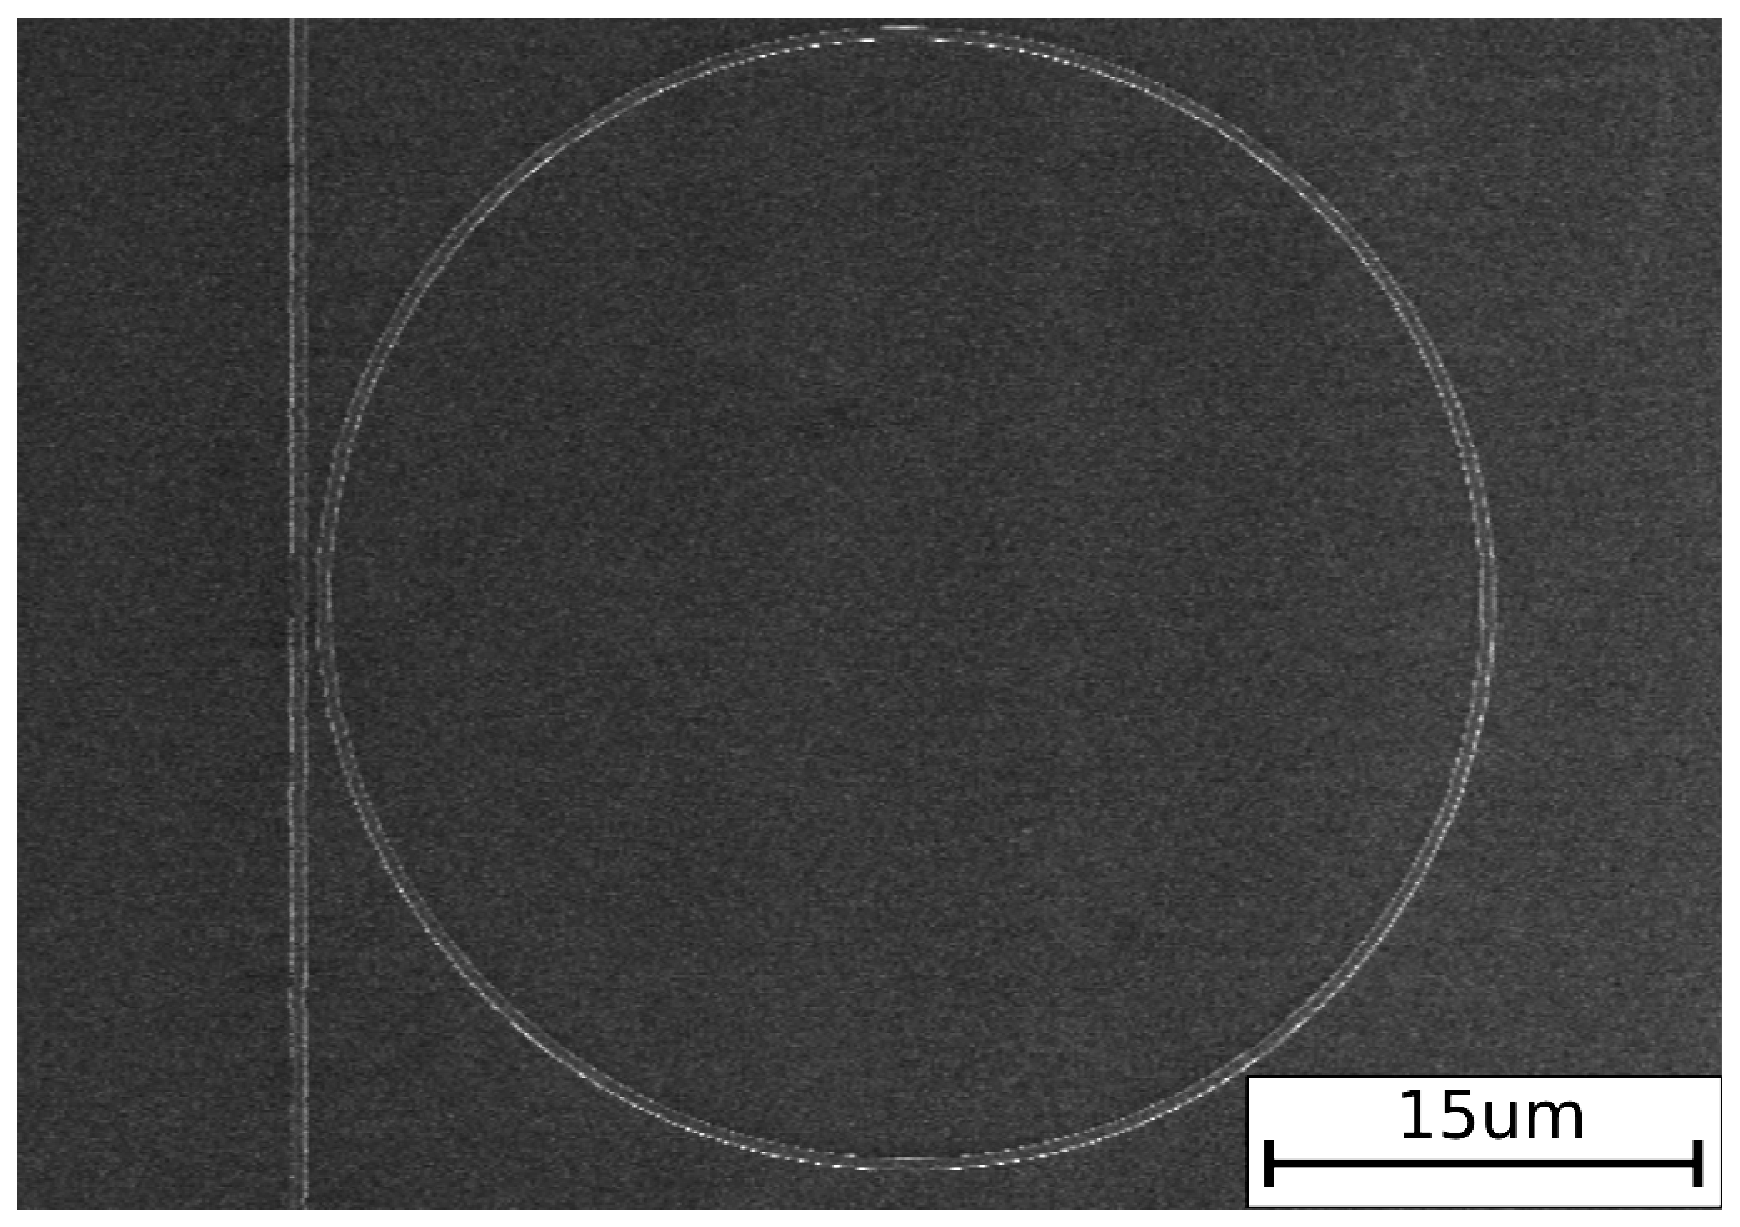
\includegraphics[width=2.5in]{ringTEscale2}
    \caption{Ring resonator SEM image.}
    \label{fig:semRingPaperRings}
\end{figure}



Amplitude and phase responses were normalized by a waveguide without ring, combined and fitted to the ring transfer function:

\begin{equation}
	H(\omega)=E_{in}/E_{out}=\mathrm{amplitude}\cdot e^{j\cdot \mathrm{phase}} = \frac{t-A}{1-tA}
\end{equation}
 

As we can see in Fig.~\ref{fig:undercoupled} we clearly see that under-coupled rings accumulate $2\pi$ phase shifts while over-coupled rings have phase fluctuations in each resonance as in Fig.~\ref{fig:overcoupled}. 

     
\begin{figure}[htb]
  \centerline{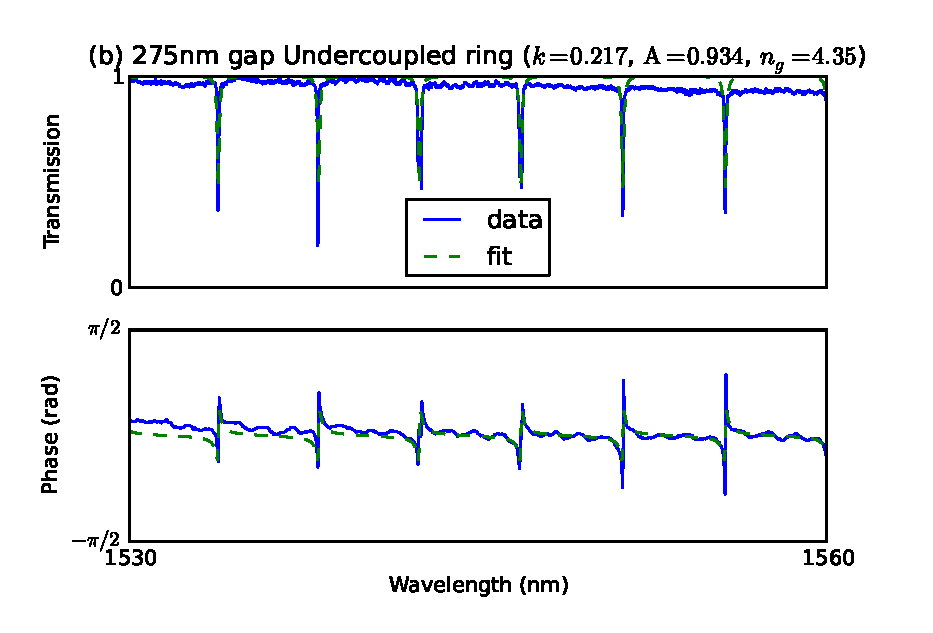
\includegraphics[width=9cm]{r20g275TE_fitPhaseAmp}}
  \caption{TE 20~$\mu$m radius and 275~nm gap ring spectrum measurement (--) and fit (-~-) for a coupling coefficient $k=0.217$, single-pass amplitude transmission $\mathrm{A=0.934}$ and group index $n_g=4.35$.}
  \label{fig:undercoupled} %[ k= 0.21659667  A= 0.93423178  neff= 4.35316758] 
\end{figure}



\begin{figure}[htb]
  \centerline{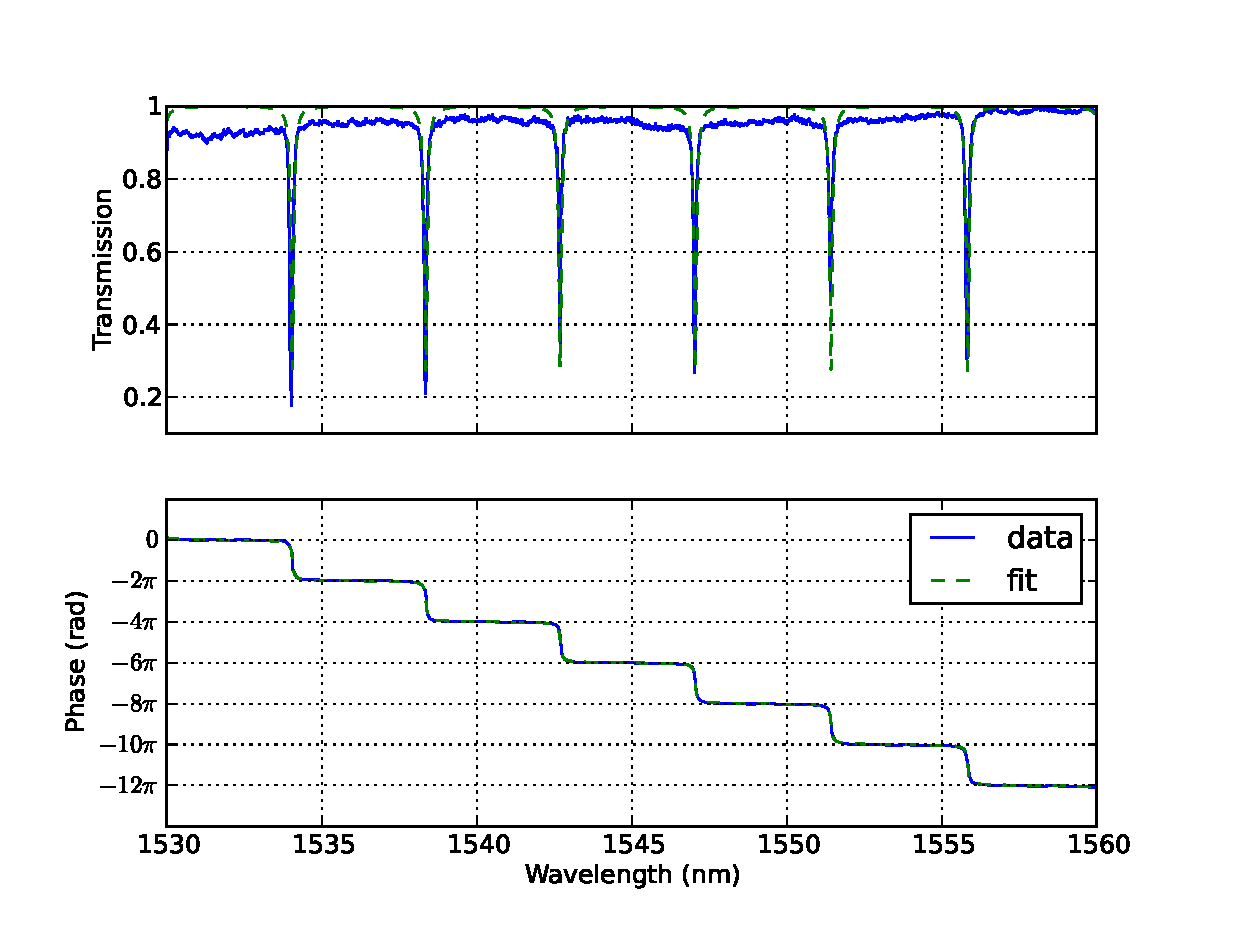
\includegraphics[width=9cm]{r20g200TE_fitPhaseAmp}}
  \caption{TE 20~$\mu$m radius and 200~nm gap ring spectrum measurement (--) and fit (-~-) for a coupling coefficient $k=0.350$, single-pass amplitude transmission $\mathrm{A=0.963}$ and group index $n_g=4.36$.}
  \label{fig:overcoupled} % [k = 0.35048909  0.96328564  4.35909895] -25.8545799362 dB/cm 
\end{figure}


\subsection{Slow light corrugated waveguides}
\label{sec:corrWaveguides}
The corrugated waveguides were designed with a flattened group index profile in a relatively broad wavelength range (from 1560 to 1610~nm), achievable by patterning circular holes onto the wide section of the waveguide as in~\cite{Brimont2010} (See Fig.~\ref{fig:sem}).


\begin{figure}[htb]
	\centering
	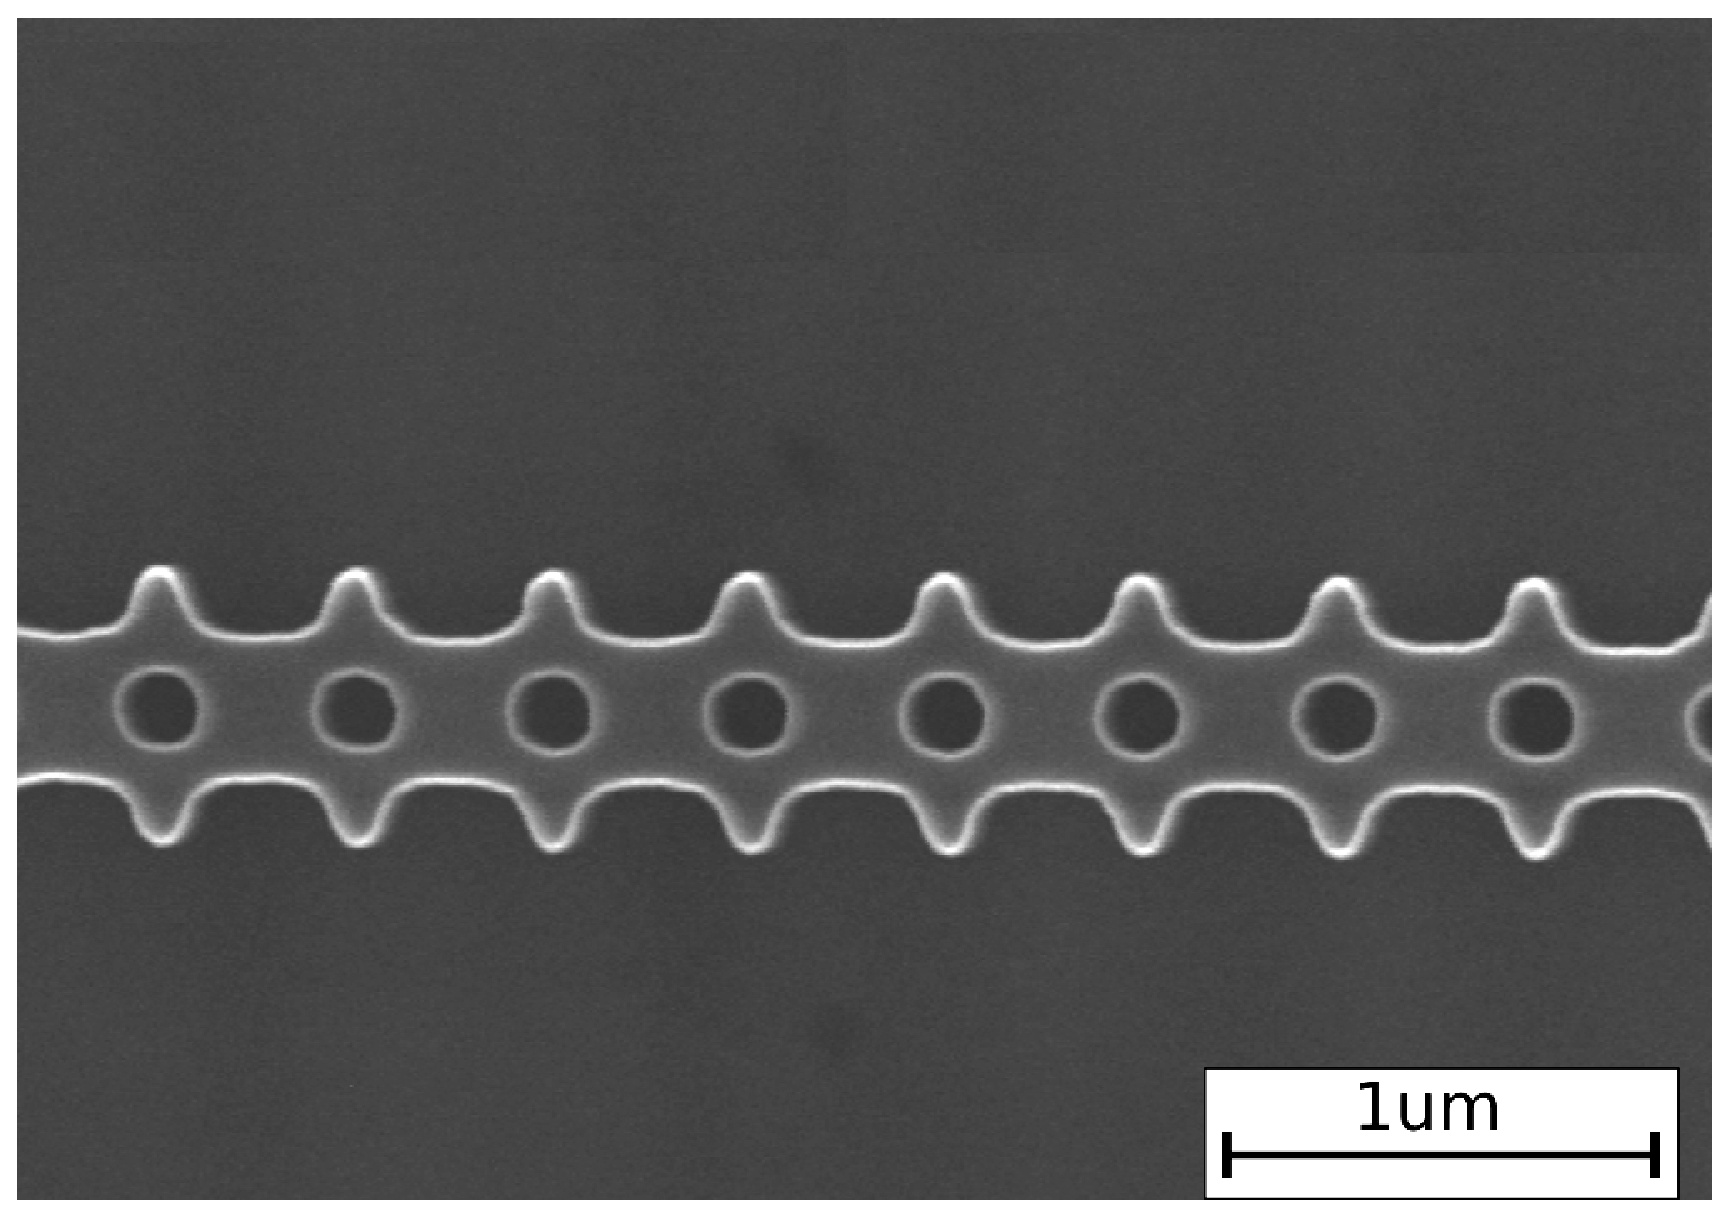
\includegraphics[width=2.5in]{corrTEscale}	
	\caption{Corrugated waveguide SEM image.}
	\label{fig:sem}
 \end{figure}



Traditional group index measurements are based on fringe separation ~\cite{shang81,vlasov:05,yao:811,Dulkeith2006} and path balancing~\cite{Cohen:82,Knox:88,Liang:98} of a Mach-Zehnder interferometer.



In Fig.~\ref{fig:groupIndex} we show the fringes of an interferometer with a 450~$\mu$m corrugated waveguide in one branch and a reference photonic wire on the other branch. From the wavelength fringe separation ($ \lambda_{min} - \lambda_{max} $) we obtain the variation of the group index with respect to the photonic wire $ n_{g,ref} $~\cite{vlasov:05}:


\begin{equation}
  n_g (\lambda)=\frac{\lambda_{min} \lambda_{max}}{ 2L (\lambda_{min} - \lambda_{max})} + n_{g,ref}
\end{equation}


where $n_{g,ref}$ is the group index of the reference branch, which in our case was obtained from the free spectral range (FSR) of the ring resonators (Eq.~\ref{eq:FSRanillo}).  % $n_{g,ref}=4.36$


On the other hand, our technique provides a continuous phase characterization from which we can extract group index with high resolution only limited by the laser step size.

We characterized and subtracted the phase evolutions of a 450~$\mu$m and a 27~$\mu$m corrugated waveguide to obtain the phase evolution of a 423~$\mu$m waveguide without the system response. To balance our interferometer from the short (27~$\mu$m) to the long (450~$\mu$m) waveguide, a 11~ps delay increment was necessary in the optical-delay-line (ODL). This means that an equivalent $L=423~\mu$m-long corrugated waveguide has a group delay $T_g=11$~ps, which corresponds to a group index $n_g(\omega_0)=7.8$ (Eq.~\ref{eq:group_index_pathBalancing}). With the balanced interferometer  we obtained the group index variations around $n_g(\omega_0)$ from the phase evolution differential~(Eq.~\ref{eq:groupIndexEvolution}, Fig.~\ref{fig:groupIndex}):

\begin{equation}
  n_g (\omega)=  n_g(\omega_0) + \frac{c}{L} \frac{d\phi}{d\omega}
 \label{eq:groupIndexEvolution}
\end{equation}



\begin{figure}[htb]
  \centering
  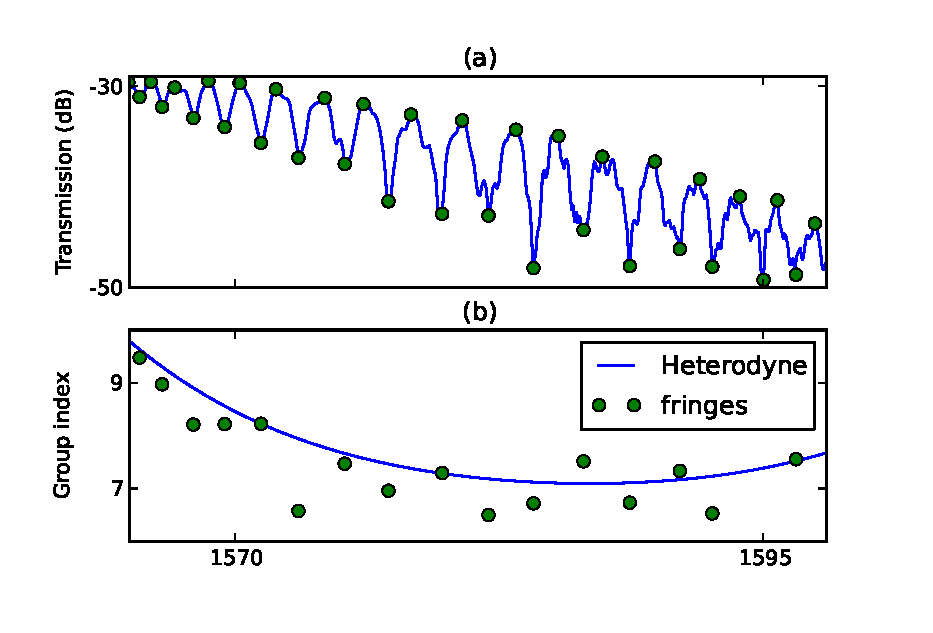
\includegraphics[width=3.5in]{gropIndexComparison_2}
  \caption{In blue dashed line: continuous group index measurement. In green dots, traditional group index measurement using an indirect measurement of the phase with the fringes of a MZI interferometer. Fringes get narrower at the band edges of the corrugated waveguide, known as slow light region, where we observe higher group index ($n_g$).} 
  \label{fig:groupIndex}
\end{figure}



\section{Conclusion}
We have shown an experimental technique for phase response characterization of integrated photonic components. The technique cancels out phase noise by using a counter-propagating reference beam, thus avoiding the need of extremely fast tuning rates or cumbersome temperature control schemes. Two components, a microring resonator and a corrugated waveguide were characterized as examples of application. From the ring resonator results, overcoupling and undercoupling regimes were clearly distinguished from the phase response and excellent agreement with simulations was observed. In the corrugated waveguide, the group index profile in the slow-light band was measured with better resolution than with a traditional fringe-spacing method.


\section*{Acknowledgments}
We acknowledge financial support from the Spanish Ministry of Science and Innovation through contracts SINADEC (TEC2008- 06333) and PROMETEO/2010/087 NANOFOTONICA. Joaquin Matres is supported by a doctoral grant of the Universidad Polit\'ecnica de Valencia. We also acknowledge Binbin Guan for fruitful discussions and Jose Angel Ayucar and Javier Garcia-Castello for help taking the SEM pictures.


% Generated by IEEEtran.bst, version: 1.13 (2008/09/30)
\begin{thebibliography}{10}
\providecommand{\url}[1]{#1}
\csname url@samestyle\endcsname
\providecommand{\newblock}{\relax}
\providecommand{\bibinfo}[2]{#2}
\providecommand{\BIBentrySTDinterwordspacing}{\spaceskip=0pt\relax}
\providecommand{\BIBentryALTinterwordstretchfactor}{4}
\providecommand{\BIBentryALTinterwordspacing}{\spaceskip=\fontdimen2\font plus
\BIBentryALTinterwordstretchfactor\fontdimen3\font minus
  \fontdimen4\font\relax}
\providecommand{\BIBforeignlanguage}[2]{{%
\expandafter\ifx\csname l@#1\endcsname\relax
\typeout{** WARNING: IEEEtran.bst: No hyphenation pattern has been}%
\typeout{** loaded for the language `#1'. Using the pattern for}%
\typeout{** the default language instead.}%
\else
\language=\csname l@#1\endcsname
\fi
#2}}
\providecommand{\BIBdecl}{\relax}
\BIBdecl

\bibitem{Vanwiggeren2003}
\BIBentryALTinterwordspacing
G.~D. VanWiggeren, A.~R. Motamedi, and D.~M. Barley, ``{Single-scan
  interferometric component analyzer},'' \emph{Photonics Technology Letters,
  IEEE}, vol.~15, no.~2, pp. 263--265, 2003. [Online]. Available:
  \url{http://ieeexplore.ieee.org/xpls/abs\_all.jsp?arnumber=1174140}
\BIBentrySTDinterwordspacing

\bibitem{Gifford2005}
D.~K. Gifford, B.~J. Soller, M.~S. Wolfe, and M.~E. Froggatt, ``{Optical vector
  network analyzer for single-scan measurements of loss, group delay, and
  polarization mode dispersion},'' \emph{Applied optics}, vol.~44, no.~34, pp.
  7282--7286, 2005.

\bibitem{Mas2012}
S.~Mas, J.~Matres, J.~Marti, C.~J. Oton, and J.~Mart\'{\i}, ``{Accurate
  chromatic dispersion characterization of photonic integrated circuits},''
  \emph{Photonics Journal, IEEE}, vol.~4, no.~3, pp. 825--831, Jun. 2012.

\bibitem{Bogaerts:12}
\BIBentryALTinterwordspacing
W.~Bogaerts, P.~{De Heyn}, T.~{Van Vaerenbergh}, K.~{De Vos}, S.~{Kumar
  Selvaraja}, T.~Claes, P.~Dumon, P.~Bienstman, D.~{Van Thourhout}, and
  R.~Baets, ``{Silicon microring resonators},'' \emph{Laser \& Photonics
  Reviews}, vol.~6, no.~1, pp. 47--73, 2012. [Online]. Available:
  \url{http://dx.doi.org/10.1002/lpor.201100017}
\BIBentrySTDinterwordspacing

\bibitem{McKinnon2009}
\BIBentryALTinterwordspacing
W.~R. McKinnon, D.~X. Xu, C.~Storey, E.~Post, a.~Densmore, a.~Del\^{a}ge,
  P.~Waldron, J.~H. Schmid, and S.~Janz, ``{Extracting coupling and loss
  coefficients from a ring resonator.}'' \emph{Optics express}, vol.~17,
  no.~21, pp. 18\,971--82, Oct. 2009. [Online]. Available:
  \url{http://www.ncbi.nlm.nih.gov/pubmed/20372631}
\BIBentrySTDinterwordspacing

\bibitem{Brimont2010}
\BIBentryALTinterwordspacing
A.~Brimont, J.~V. Gal\'{a}n, J.~M. Escalante, J.~Mart\'{\i}, and P.~Sanchis,
  ``{Group-index engineering in silicon corrugated waveguides.}'' \emph{Optics
  letters}, vol.~35, no.~16, pp. 2708--10, Aug. 2010. [Online]. Available:
  \url{http://www.ncbi.nlm.nih.gov/pubmed/20717431}
\BIBentrySTDinterwordspacing

\bibitem{shang81}
H.-T. Shang, ``{Chromatic dispersion measurement by white-light interferometry
  on metre-length single-mode optical fibres},'' \emph{Electronics Letters},
  vol.~17, no.~17, pp. 603--605, 1981.

\bibitem{vlasov:05}
Y.~A. Vlasov, M.~O'Boyle, H.~F. Hamann, and S.~J. McNab, ``{Active control of
  slow light on a chip with photonic crystal waveguides},'' \emph{Nature}, vol.
  438, no. 7064, pp. 65--69, 2005.

\bibitem{yao:811}
\BIBentryALTinterwordspacing
X.~S. Yao and J.~Feinberg, ``{Simple in-line method to measure the dispersion
  of an optical system},'' \emph{Applied Physics Letters}, vol.~62, no.~8, pp.
  811--813, 1993. [Online]. Available:
  \url{http://link.aip.org/link/?APL/62/811/1}
\BIBentrySTDinterwordspacing

\bibitem{Dulkeith2006}
\BIBentryALTinterwordspacing
E.~Dulkeith, F.~Xia, L.~Schares, W.~M.~J. Green, L.~Sekaric, and Y.~A. Vlasov,
  ``{Group index and group velocity dispersion in silicon-on-insulator photonic
  wires.}'' \emph{Optics express}, vol.~14, no.~13, p. 6372, Jun. 2006.
  [Online]. Available:
  \url{http://www.opticsinfobase.org/abstract.cfm?\&amp;id=89589
  http://www.ncbi.nlm.nih.gov/pubmed/19516814}
\BIBentrySTDinterwordspacing

\bibitem{Cohen:82}
L.~G. Cohen and J.~Stone, ``{Interferometric measurements of minimum dispersion
  spectra in short lengths of single-mode fibre},'' \emph{Electronics Letters},
  vol.~18, no.~13, pp. 564--566, 1982.

\bibitem{Knox:88}
\BIBentryALTinterwordspacing
W.~H. Knox, N.~M. Pearson, K.~D. Li, and C.~A. Hirlimann, ``{Interferometric
  measurements of femtosecond group delay in optical components},'' \emph{Opt.
  Lett.}, vol.~13, no.~7, pp. 574--576, Jul. 1988. [Online]. Available:
  \url{http://ol.osa.org/abstract.cfm?URI=ol-13-7-574}
\BIBentrySTDinterwordspacing

\bibitem{Liang:98}
\BIBentryALTinterwordspacing
Y.~Liang and C.~P. Grover, ``{Modified white-light Mach-Zehnder interferometer
  for direct group-delay measurements},'' \emph{Appl. Opt.}, vol.~37, no.~19,
  pp. 4105--4111, Jul. 1998. [Online]. Available:
  \url{http://ao.osa.org/abstract.cfm?URI=ao-37-19-4105}
\BIBentrySTDinterwordspacing

\end{thebibliography}

% \bibliographystyle{IEEEtran}
% \bibliography{/home/joaquin/Documents/library}
\end{document}

